\newpage
\section{Detailed Implementation}
\label{section:implementation}
Please explain your implementation in detail. You may do this with the help of pseudo code or a figure of system architecture. Please also highlight which parts of the algorithm lead to the most difficulty in your implementation.


\subsection{Whole iRDPG Algorithm}
iRDPG proposed by \cite{liu2020adaptive} is abbreviation of imitative Recurrent Deterministic Policy Gradient. As the name suggests, which improve RDPG by introducing imitation learning. 

As the figure showed bellow. We can see the architecture of iRDPG. The bottom part is the market observation.  It will first be fed into the GRU layer to encode its historical information, and then the GRU hidden state will be send into the Agent. In the agent module, the behavior cloning loss is used to supervised the actor. And the Demonstration Buffer allows Actors to learn the experience of expert.

\begin{figure}[h!]
    \center
    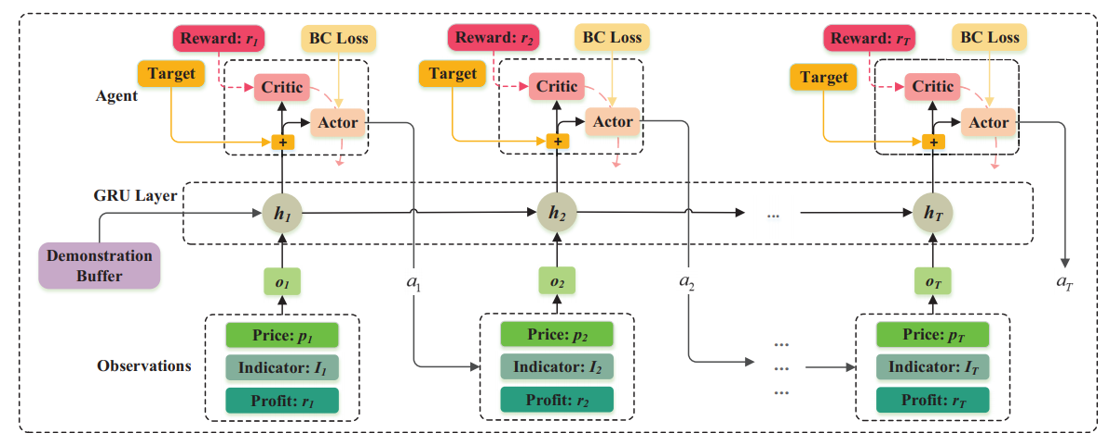
\includegraphics[width=14cm]
    {irdpg}
    \caption{The overview of iRDPG model}
    \label{fig: The iRDPG model}
\end{figure}



\subsection{Experiment Setup}
In our experiment, we use minute-bar OHLC prices data of futures, 
i.e. minute-frequent futures data(IF and IC) \cite{joinQuant}. \\
Training set starts from 2016/01/01 to 2018/05/08. \\
Testing set spans from 2018/05/09 to 2019/05/08. \\
Transaction fee  : 2.3*10-5 \\
The constant slippage: 0.2 \\
Initialize account: 500000 CNY\\
Each training episode will be broken off once positions are lost around 30\% or lacking margin.

\begin{figure}[h!]
    \center
    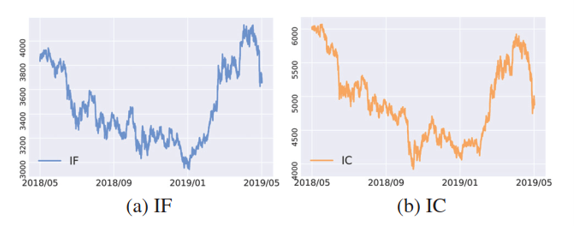
\includegraphics[width=10cm]
    {IFIC_2}
    \caption{ IF and IC stock-index futures in our test set}
    \label{fig: The IF IC}
\end{figure}

* The IF data are based on the index calculated on account of the prices of the top 300 stocks from both 
Shanghai and Shenzhen exchange centers. \\
* The IC data are based on another similar index, which focuses on the stocks with mid and small capitalization. \\


\subsection{Dual Thrust Strategy}

It is famous and has been commonly used in futures, forex, and equity markets.
As the introduction in the Demonstration Buffer, we select the Dual Thrust strategy as the demonstration trading policy. First, the DT determines a reasonable price oscillation Range, and the Range is calculated in this way by using OHLC in the previous n periods.
Then use this range to determine the buyline and sellline. Finally, if the price goes beyond the buyline, a long position will be taken.
And the short position will be taken if the price goes under the sellLine.

The long signal is calculated by Buyline (cap)=open+K1×Range. \\
The short signal is calculated by SellLine (floor) = open–K2×Range \\
, where K1 and K2 are the parameters. When K1 is greater than K2, it is much easier to trigger the long signal and vice versa. 
The idea of Dual Thrust is similar to a typical breakout system, However, dual thrust uses the historical price to construct update the look back period - theoretically making it more stable in any given period.


\begin{figure}[h!]
    \center
    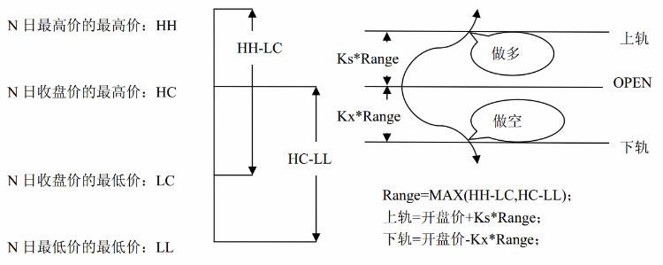
\includegraphics[width=12cm]
    {DT_1}
    \caption{Dual Thrust Strategy}
    \label{fig: The DT1}
\end{figure}

% \begin{figure}[h!]
%     \center
%     \includegraphics[width=10cm]
%     {DT_2}
%     % \caption{Dual Thrust Strategy}
%     \label{fig: The DT2}
% \end{figure}

\subsection{The Most Difficulties in Our Implementation}
First, no member is familiar with the market characteristics and trading rules of China stock index futures, but fortunately the minute-frequent price data can be friendly downloaded on JoinQuant website for a student registration member. 
Beside, although the POMDP framework can better represent the noisy minute-frequent financial data, it is still quite a challenge to tune the agent. \\
No source code, the simulated trading environment is also coded from scratch, its complexity is beyond our imagination. Besides, although the differential sharp ratio (DSR) looks having nice property for considering both dynamically changing return and risk, but the formula often faces zero values for both numerator and denominator and how to set the proper value of adaptation rate $\eta$.\\
The ablation experiment takes so much time because the hyperparameters are quite different for each setting. For example, when adding the new imitation techniques to the original RDPG, the characteristics for each training process are very different, the trial and error need much efforts. \\





